% illustrer les performances ainsi que l'efficacité du logiciel implémenté
% a l'aide de graphiques.


% analyser (et comparer, si plusieurs) les performances des solutions 
% implémentées


% présenter les bancs d'essais (ou les procédures utilisées pour la génération)
% des données) utilisés pour les tests du logiciel.

\section{Algo MinMax observations}
Une fois l'implémentation de l'algorithme MinMax faite sur nos deux
jeux combinatoires, nous pouvons nous demander est-ce que cet algorithme est adapté pour le jeu de Hex et l'Awale ?
Nous observons que les performances du MinMax sont très différentes d'un jeu a l'autre, étudions pourquoi:

\subsection {Hexgame : performances décevantes}
L'implémentation de l'algorithme MinMax sur le jeu de Hex n'arrive quasiment jamais à battre un humain et cela pour 
2 raisons principales: la faible profondeur et la difficulté de trouver une fonction d'évaluation satisfaisante.

\paragraph {Trop grande complexité} Le premier problème provient du nombre de coups possibles à chaque tour: 
en effet, par exemple sur un plateau classique de $13\times13$ le premier joueur a 169 coups possibles et au coup suivant
il y en a 168 etc\dots Cela rend les calculs lents. S'il joue en premier 
et que la profondeur demandée est de 6, alors l'ordinateur doit calculer $2.1298467e+13$ (ou $169\times168\times167\times166\times165\times164$) 
fois la fonction d'évaluation. Cela n'est pas réalisable en temps réaliste. Dans notre implémentation, la taille des côtés du plateau varie entre  
une longueur de 5 cases et de 17, nous avons remarqué que pour un plateau de dimension $11\times11$ l'algorithme mettait déjà 
plusieurs secondes à calculer le meilleur coup. Notons que ces calculs ne prennent pas en compte l'élagage alpha-bêta
qui optimise significativement le MinMax. Mais même si une portion des nœuds n'est pas évaluée, le calcul reste trop lent.
On peut aussi noter que la performance de l'élagage alpha-bêta dépend de la qualité de la fonction d'évaluation, qui, comme nous allons
le voir, n'est pas assurée.

\paragraph{Fonction d'évaluation : Un vrai casse-tête}Le MinMax n'arrivant pratiquement jamais à une feuille terminale, nous avons compris que la fonction
d'évaluation du Hex devait être performante et peu coûteuse en temps. Cependant, faire comprendre à l'ordinateur si une position est gagnante 
ou non s'est révélé difficile. En effet, le Hex est un jeu possédant de nombreuses stratégies, et relier toutes ces stratégies en une 
seule fonction d'évaluation est quelque chose de très compliqué. Ainsi, nous avons rapidement cherché à faire comprendre à l'ordinateur 
quelle stratégie adapter au fur et à mesure de la partie ? Parmi elles, la stratégie de faire des ponts (voir la figure 3) nous a posé beaucoup de problèmes.
Un pont permet au joueur de s'assurer de pouvoir connecter 2 pièces lors d'un prochain coup. En effet, si le joueur adversaire cherche à bloquer
l'une des deux cases, nous avons juste à ajouter notre jeton afin de créer un chemin entre ces deux pièces. Nous pouvons noter que lorsque la profondeur de 
réflexion du MinMax est grande, il arrive parfois à remarquer que créer un pont le meilleur coup. Mais nous revenons au problème n°1 : la complexité. 
Dans notre projet, la fonction d'évaluation finale va permettre à l'ordinateur de créer les groupes de jetons les plus grands en largeur ou en hauteur en 
fonction du joueur. Elle est capable de battre des humains sur de petits plateaux. Mais en général, lorsque le plateau est de grande dimension, la fonction
d'évaluation prend de nombreuses secondes avant de jouer.
\begin{figure}[h]
    \begin{center}
        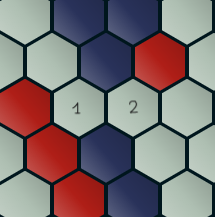
\includegraphics[scale=0.5]{root/pont.png}
    \end{center}
    \caption[1]{Ici bleu a créé un pont\footnotemark.}\label{fig:pont_bleu}
\end{figure}

\footnotetext{Si rouge joue sur la case 1, bleu joue sur la case 2, et relie ainsi les deux jetons bleus (respectivement si rouge joue sur la case 2)}



\subsection {Awale : Bonnes performances}
\paragraph {Une fonction d'évaluation efficace} Le jeu de l'Awalé possède un avantage significatif par rapport au Hex, le nombre maximum de coups 
possible pour un joueur est de 6. Ainsi, l'arbre de recherche est bien plus petit que celui du Hex. L'algorithme MinMax est donc efficace en termes de 
temps et de performances avec une grande profondeur (la profondeur initiale est de 6). 

Le choix de notre fonction d'évaluation est arrivé naturellement pendant nos recherches. Nous avons implémenté la simple fonction cherchant à
maximiser les points de l'ordinateur tout en minimisant les points de son adversaire. Cette fonction combinée à une profondeur de taille 6 en fait un 
adversaire redoutable que peu d'humains ont réussi à battre.

\paragraph {Conclusion} L'algorithme MinMax est donc capable d'être efficace lorsque le nombre de nœuds est petit à chaque itérations. On peut alors 
lui mettre une profondeur relativement grande afin d'explorer toutes les branches de cet arbre. Cependant, lorsque le nombre de nœuds devient gigantesque,
l'algorithme ne devient plus très bon. Il est en effet très lent et peu performant.